\vspace*{-0.3cm}
\section{Background and Motivation}
\vspace*{\subsecspace}
\label{sec:bg}

\subsection{Providing Functions as a Service}

Serverless computing entails executing snippets of user code, usually in an event-driven manner, inside protected and isolated sandboxes~\cite{serverless-cacm-21}.
For users, serverless functions offer many features such as elastic scaling and scale-to-zero, making cloud-native applications easier to develop and deploy. 
% As a result, FaaS has emerged as a common abstraction for a wide range of cloud services such as orchestration and workflows, IoT, machine learning and data analytics pipelines, scientific computing, etc. 
The FaaS \emph{provider} usually runs a \emph{control plane} such as OpenWhisk and OpenFaaS (or proprietary ones in the case of popular services like Amazon Lambda~\cite{aws-lambda}), for handling the scheduling, scaling, load-balancing, resource limiting, and accounting for each invocation. 

From the FaaS control plane's perspective, the popularity and diversity of FaaS workloads makes these tasks particularly challenging, and can add several dozen milliseconds of latency in orchestrating function invocations~\cite{cvetkovic2024dirigent, fuerst2023iluvatar, serverless-cluster-cost}.
Because of the richness of their usecases, function workloads are highly diverse with a range of several orders of magnitude in all dimensions.
For example, both Azure~\cite{shahrad2020serverless} and Alibaba~\cite{luo2021characterizing} workloads indicate that the inter-arrival-times can range from 0.1s to hours, the execution times can range from milliseconds to minutes, and the memory footprint from 100 MB to 5 GB. 
From the FaaS control plane point of view, an invocation is a \quotes{black-box} containerized task with known resource limits (such as the number of allocated CPUs and memory size).
Function resource usage is typically similar across invocations, and control planes also use these estimates for implementing advanced policies for keep-alive~\cite{roy2022icebreaker,faascache-asplos21}, placement, etc. 


\subsection{Why GPU Acceleration for Functions}

%1. Many applications benefit
%2. GPU hardware present on many servers anyways. Thus need the opportunistic acceleration. 
\begin{comment}
\mhead{Serverless Use Cases}
The number of serverless use cases than use or can benefit from acceleration is continuously growing.
Encoding of videos~\cite{ao2018sprocket, zhang2019video} and analytics on live video streaming~\cite{romero2021llama, risco2021gpu} are ideal for both FaaS scaling and internal application parallelism. 
% Machine learning in all its forms has made its way into the serverless research.
% Commonly to make scheduling decisions for containers~\cite{balaji2021fireplace} or resource allocation to them~ \cite{mvondo2021ofc,eismann2021sizeless}.
Machine learning inference has need for low-latency results, and has seen much work in serverless~\cite{yang2022infless, ali2022optimizing, ali_batch_2020}, and can achieve lower latency with acceleration.
% And finally are works that do training, taking advantage of the serverless scaling~\cite{wang2019distributed, gimeno2022mlless, xu2021lambdadnn}.
%
The exposure of supercomputing resources to run scientific workloads by~\cite{funcx_hpdc_20} highlights the demand for parallelization of functions.
Such science workloads vary from biomedical research~\cite{kumanov2018serverless,hung2019rapid}, linear algebra~\cite{werner2018serverless,shankar2020serverless}, to optimization algorithms~\cite{aytekin2019harnessing}.
\end{comment}

\begin{table}
  \caption{Latencies (in seconds) for GPU and CPU \textbf{W}arm and \textbf{C}old functions.}
  \label{tab:gpu-cpu}
  \vspace{\captionspace}
  % \begin{center}
  \begin{tabular}{lccc}
    \hline
    Function & GPU [\textbf{W}] & CPU [\textbf{W}] & GPU [\textbf{C}] \\
    \hline
  Imagenet [ML] & 2.253 & 5.477 &     8.581 \\
  Roberta [ML] & 0.268 & 5.162 &     16.374 \\
  Ffmpeg [Video] & 4.483 & 32.997 &     12.044 \\
  FFT [HPC] & 0.897 & 11.584 &     2.648 \\
  % Eos & 0.017 & 0.045 & 2.66x \\
  Isoneural [HPC] & 0.026 & 0.501 &     2.586 \\
  % Lavamd & 1.989 & 15.199 & 7.64x \\
  Lud [Rodinia] & 2.050 & 70.915 &     2.125 \\
    Myocyte [Rodinia] & 2.784 & 39.277 &      2.145 \\
  Needle [Rodinia] & 1.979 & 144.639 &     2.292 \\
  Pathfinder [Rodinia] & 1.472 & 134.358 &     1.997 \\
  % Srad & 3.893 & 119.759 & 30.77x \\
  \end{tabular}
% \end{center}
  \vspace{-0.4cm}
\end{table}

% One of the first works to integrate GPUs is~\cite{naranjo2020accelerated} using rCUDA~\cite{duato2010rcuda} to connect disaggregated GPUs in a cluster to containers.
% It only looks at the performance affect on individual function invocations, not exploring the resource management, queuing, or heterogeneous load issues in FaaS.
% DGSF~\cite{fingler2022dgsf} combines disaggregation and API remoting to improve utilization, and does load-balancing between GPUs on the compute node.


Many applications that have adopted FaaS for its on-demand scaling also benefit from GPU acceleration, as shown by Table~\ref{tab:gpu-cpu}, where we compare the execution times of functions using an NVidia V100 GPU and an Intel Xeon Gold 3.2 GHz CPU.
CPU functions are allocated one CPU core, and GPU functions can use the entire accelerator.
Machine learning inference tasks such as Imagenet and Roberta see a 3x and 20x reduction in latency compared to a warm CPU container. 
Video encoding via \emph{ffmpeg}, which is one of the most popular functions on AWS Lambda~\cite{aws-netflix}, can also leverage specialized hardware found in most GPUs for a 7x speedup. 
Scientific computing has started to be used in FaaS~\cite{john_sweep_2019,mocskos_faaster_2018,werner2018serverless,shankar2020serverless}, and also benefits from GPU acceleration for its common primitives such as FFT.
%One such ubiquitious algorithm, Fast Fourier Transform (FFT), sees 13x improvement, and larger, complete applications (Needle, Pathfinder, etc.) are 80-90x faster with acceleration. 


Thus a large class of FaaS workloads are potentially amenable to GPU acceleration.
The serverless abstraction allows decoupling of computation from its location, and prior work has investigated the use of remote disaggregated GPUs for FaaS~\cite{naranjo2020accelerated,fingler2022dgsf}, and providing acceleration as a service~\cite{varghese2015acceleration,du2022serverless}.
%These prior efforts have focused on the virtualization of accelerators through new mechanisms and abstractions, and often for specialized workloads such as ML inference.
%We focus on a higher level of abstraction, and develop scheduling policies for providing GPU acceleration \emph{at scale} which can be integrated as part of a high-performance FaaS control plane.
Serverless functions in public cloud with enabled GPUs have started to appear~\cite{azure-gpu-function,alibaba-gpu-function}, but are far from ideal.
These use GPU-passthrough techniques~\cite{alibaba-gpu-noshare}, which statically allocate hardware and have low utilization, and sometimes one must even self-host the hardware~\cite{azure-gpu-function}.

% \todo{Add refs for azure and alibaba gpu functions and describe how they are limited/different. See \cite{sage_zhao_towards_2024} for these refs.}

\vspace*{\subsecspace}
\subsection{GPU Programming Model}
%TODO: Integrate with previous (gpu support for functions)

Applications cannot usually manipulate GPUs directly, and must use a manufacturer-provided driver for all operations.
Host programs launch \emph{kernels} which execute a code block with given memory inputs and a number of parallel threads to use.
Multiple kernels can be launched concurrently, with the device handling scheduling of kernels and threads internally.
Kernels run until completion, with execution time varying widely depending on the number of threads, input size, and complexity of the code being run. 
Traditionally, programs manually move data between the host and device (using \funcname{cuMemAlloc} for instance).
Virtualizing GPU memory (by using CUDA's Unified Virtual Memory (UVM)~\cite{nvidia-uvm}) allows memory overcommittment, which is important for supporting high degrees of multiplexing.
% Programs allocate memory using \funcname{cuMemAllocManaged} instead of \funcname{cuMemAlloc}, and the device driver moves memory between the device and host in response to usage and memory pressure.
%When using \funcname{cuMemAllocManaged}, the same memory pointer can be used on both host and device, and the driver is responsible for data migration and coherency.
%This capability is also used by UVM to allow over-subscription of memory, as it will move data pages around on-demand, using host memory as \quotes{swap} space. 
%We integrate our control plane with UVM to actively oversubscribe memory, allowing many function containers to remain warm on a device without interference, dramatically reducing cold starts. 

For multiplexing functions on GPUs, the naive approach entails fully assigning the GPU to a function. 
Because functions are short-lived (at most a few minutes), we can use the GPU in an FCFS run-to-completion model. 
However, this leads to poor GPU utilization since functions are often small and will not use all GPU resources, and also highly detrimental for function latency due to cold-starts, as we explain in the next section. 
A typical FaaS server runs 10--50 functions concurrently, and thus even if a small fraction of them can benefit from GPU acceleration, an immediate need arises for multiplexing the GPU to run multiple functions concurrently. 
However, GPUs have conventionally been designed for high throughput computation for a single long-running application, which is reflected in their hardware architecture and software stacks.
The performance-first focus has also resulted in many cross-layer optimizations which make multiplexing and virtualization challenging. 


% , regardless of the function it is for.
% The amount of GPU memory and compute usable by a process can be specified at process launch time, and is fixed thereafter.
% Importantly, support for MPS features varies between hardware versions, and only the newest devices have resource management features.
% Both spatial approaches have drawbacks that render them unsuitable for FaaS.

% Resource partitioning, a new container must be spun up with the large overhead that entails.
% MPS does not enable oversubscribing limited device memory, and the inability to truly isolate processes from one another makes it a poor candidate for FaaS.
% Both spatial sharing schemes do not allow variable resource allocations, requiring a container cold start to change allocations.
% Neither enable oversubscription of limited device memory, 


\begin{comment}
\mhead{Memory Multiplexing}
Limitations caused by requiring driver interaction to control the device makes it a challenge to multiplex memory.
Virtualization approaches~\cite{yu2019automatic, hong2017gpu} must duplicate application state in host memory, and allocate/de-allocate all resources when switching between applications.
Kernel level schedulers~\cite{ng2023paella,pemberton2022kernel,strati2024orion} are able to manipulate and oversubscribe memory as any GPU application would, but violate the black-box principles we target.
Interposition and disaggregation techniques~\cite{duato2010rcuda,fingler2022dgsf} allow for true multiplexing similar to our design, thanks to their level of control equal to that of a kernel scheduler while not being part of the actual application.
\end{comment}

\vspace*{\subsecspace}
\section{Design Requirements and Key Challenges}
\label{sec:motiv}

Our work considers discrete and integrated GPUs, and our task is to provide \emph{opportunistic} GPU acceleration to functions that benefit from it.
We assume a classic, non-disaggregated hardware platform where the GPU functions can run locally. 
Due to the surge of ML workloads, discrete and integrated GPUs are a common feature in data center and even edge clusters. 
For example, the popular Nvidia Jetson Orin platform provides more than 60\% of its compute capabilities (FLOPS) in the integrated GPU.
% \todo{Check FLOPS}
Since FaaS is the common abstraction for supporting a wide range of applications, we seek a general-purpose \emph{black-box} solution which supports arbitrary functions on heterogeneous clusters, and preserves existing resource isolation guarantees. 
This requires us to support different GPU usage patterns, and prevent the use of application-specific performance optimizations (such as for ML inference). 
For the FaaS hardware, we make minimal assumptions in terms of feature availability, and assume that the underlying cluster is a mix of servers with different GPU types, and support both data center and edge computing devices. 
Given all these requirements, the performance objective is to increase server utilization by running functions on GPUs, and reducing the overall function latency of FaaS workloads. 
The above constraints imposed by black-box FaaS workloads and GPU multiplexing also restrict the space of mechanisms and optimizations, which lead to the challenges described below. 


%Yet any function with a dataset that exceeds these limits or a problem space that needs parallel computing for timely results cannot be served.

\subsection{Cold-starts for GPU Containers}

\begin{figure}
  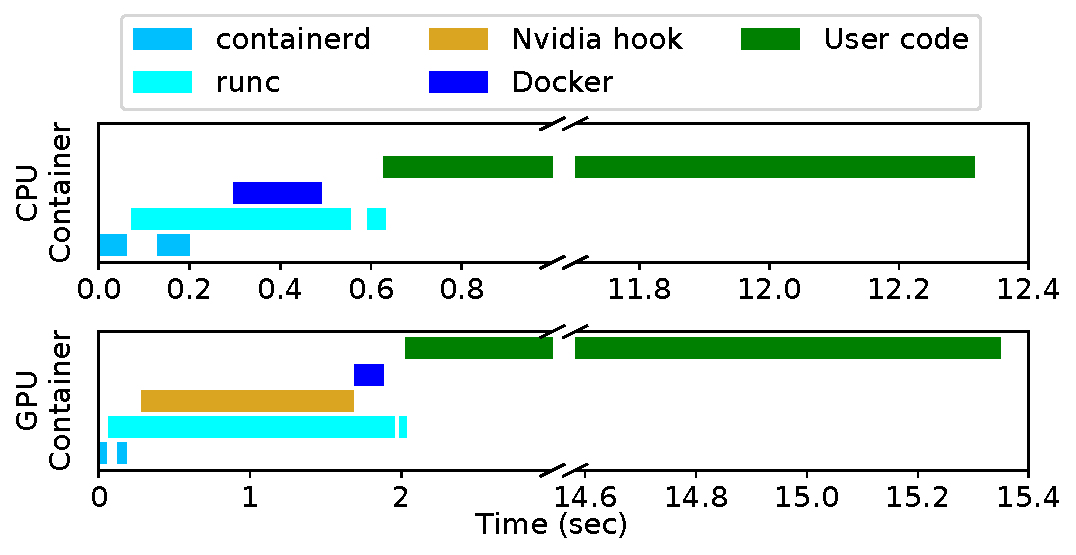
\includegraphics[width=0.45\textwidth]{../graphs/coldstart/combined_timeline.pdf}
  \vspace*{-0.35cm}
  \caption{Timeline of cold-starts of CPU (top) and GPU (bottom) function containers running TensorFlow inference code. 
    % Several additional seconds are caused by Nvidia runtimes and user code library loading.
    GPU initialization and code dependencies increase latency by three seconds.}
    \label{fig:cold-timeline}
% Gunicorn & library load time, no GPU:
% gunicorn: 0:00:11.688722
% Gunicorn & library load time, GPU:
% gunicorn: 0:00:13.320342
% nvidia: 0:00:01.399233
\vspace*{-0.3cm}
\end{figure}

Cold-starts due to sandbox creation and initialization are a well known performance problem for serverless functions~\cite{du2020catalyzer,lin_mitigating_2019,manner_cold_2018,mohan_agile_2019}.
We find that such cold starts are severely exacerbated by GPU containers, increasing latency by $1.1-75\times$ (Table~\ref{tab:gpu-cpu}).
A breakdown and comparison of these overheads for the ML inference function (using TensorFlow) is shown in Figure~\ref{fig:cold-timeline}.
For the GPU container (bottom figure), the Nvidia hook library adds more than 1.5 seconds of delay.
% , even before counting time taken by the application for initializing the GPU and loading specialized libraries.
% has the accelerator and spends roughly 1.5 seconds in an Nvidia library hook that performs kernel work to attach the GPU to the container.
User function code loads additional GPU libraries and dependencies, and its startup requires 1.5 additional seconds.
% lol not gonna do. TF does magic/BS loading of different stuff when a GPU is detected.
% \todo{Add which libraries.}

\subsection{Tradeoffs in Locality, Throughput, and Fairness}

A common approach to alleviate cold starts is to keep the container warm~\cite{faascache-asplos21} in memory.
This is also applicable for GPU containers, but with additional challenges.
First, a warm container holds GPU memory which is much more limited (e.g., the V100 has 16 GB VRAM), which reduces keep-alive's effectiveness~\cite{faascache-asplos21}, and reduces the number of containers able to be kept warm.
Additionally, the number of concurrently executing functions should also be kept low to mitigate performance interference, which can be excessive from both compute~\cite{yamagiwa2009performance,phull2012interference} and data movement between host and device~\cite{yu2019automatic, hong2017gpu}.
This reduction in concurrency increases queue waiting times.
Finally, since function workloads are highly heterogeneous and dynamic, we must select the \quotes{active} functions carefully so as to balance fairness and throughput.
% The scheduling is also affected by the high cost of data movement between host and device~\cite{yu2019automatic, hong2017gpu}.


In other contexts, application switching costs have been reduced through batching.
For example, an ML inference task can be given multiple inputs simultaneously as a batch---significantly improving throughput and utilization~\cite{ali_batch_2020,yang2022infless,ali2022optimizing}.
%The inputs of multiple invocations are merged into one \emph{batch} by the control plane, computed together, and split apart to distribute results.
% Scientific applications among others are not amenable to batching, and for those that do, they require changing the FaaS paradigm.
Such specialized and white-box solutions eschew isolation by making assumptions about the workload, such as the ability to modify the function code and input/output processing. 
For a general FaaS service, we need to provide locality improvements using a black-box approach.


Maximizing for locality entails large batches, which increases latency for both the batched function and also the other functions due to monopolization of GPU resources.  
For heterogeneous and dynamic FaaS workloads, batching policies are also significantly more challenging outside more specialized workloads like inference-as-a-service.
For example, popular functions see $100\times$ the average number of invocations, which can cause the rest of the long tail of functions to have exacerbated waiting times in the queue, leading to unfairness. 
Thus, while locality is useful for performance, it may lead to unfairness. 

\subsection{GPU Multiplexing Mechanisms}

While many hardware- and software-level virtualization and multiplexing solutions exist, they are ill-suited for the highly dynamic and heterogeneous containerized function workloads.
%\mhead{Temporal Multiplexing}
The conventional approach is to dispatch multiple GPU compute kernels (corresponding to different functions) concurrently, and let the GPU driver and hardware manage the sharing of GPU compute cores and memory.
The GPU driver itself accepts individual compute \emph{kernels} from applications and has a device-internal scheduler which maps them to available compute blocks as they arrive. 
This is one of the main mechanisms behind classic GPU virtualization work~\cite{duato2010rcuda, yu2019automatic, hong2017gpu}, but comes with significant performance overheads~\cite{yu2017full}. 
These GPU virtualization approaches duplicate application state in host memory, and allocate/de-allocate all resources when switching between applications. 
% , and most target disaggregation~\cite{duato2010rcuda,fingler2022dgsf} or API imposition~\cite{yu2019automatic}.
% These support memory and compute sharing 


\emph{Application-specific} optimizations for scheduling and multiplexing of GPU kernels can be performed at several levels of the GPU software-hardware stack. 
% Replacement schedulers~\cite{mccoy2024gallatin} have been devised, as well as systems that schedule kernel launches from inside an application~\cite{strati2024orion}.
Kernel schedulers for domain-specific optimizations~\cite{strati2024orion,chen2017effisha,kim2020navigator,gu2023fast} have been designed to coordinate kernels from several applications to improve on device scheduler performance.
These operate only on compute kernels to prevent contention and assume active concurrent workloads are coordinated elsewhere to not exceed the device memory. 
% At the highest level, a process or job can be scheduled on a specific GPU and allowed to run to completion, accepting the application's arbitrary kernel launches. 
% As many workloads can't consume all available GPU resources, some schedulers control both kernel launches and device memory.
Application-optimized and integrated scheduling solutions have recently been developed~\cite{ng2023paella,pemberton2022kernel,strati2024orion}, which interpose on the application's kernel launches.
For example, the structure of ML inference applications can be used for injecting kernel preemption code into the applications via TVM transformations~\cite{han2022microsecond} for decreasing head of line blocking and improving GPU utilization.


%include manipulating and oversubscribing memory as they schedule kernel launches, but they violate the black-box principles we target by breaking apart the application to have tighter control.
%Interposition and disaggregation techniques~\cite{fingler2022dgsf,duato2010rcuda} allow for multiplexing memory and compute similar to our design, thanks to the level of control gained by replacing the GPU driver, and are black-box because they do not replace the actual application.


GPU compute cores and memory can also be \emph{spatially partitioned} across clients/kernels using more modern GPU virtualization functionality. 
% via virtualization that vary with different hardware generations.
% Virtualization passthrough of vGPUs~\cite{nvidia-passthrough} uses direct device assignment common to hardware virtualization, where a guest VM has total control of the device with no sharing. 
Nvidia MIG~\cite{nvidia-mig} (Multi-Instance GPU) pre-partitions device resources, and one or more of these virtualized GPU partitions can be assigned to a VM or container via direct device assignment.
However, the slices are of pre-determined sizes, making them ill-suited to fine-grained and dynamic workloads~\cite{li2022miso}. 
Similarly, Multi-Process Service~\cite{nvidia-mps} (MPS) allows multiple processes to make share the device concurrently and has been proposed for FaaS~\cite{gu2023fast}.
An MPS server and the hardware device perform resource partitioning based on configuration at application start time.
MPS is explicitly designed to let cooperative processes share GPU resources, and documentation specifies that it is intended to work with OpenMP/MPI applications~\cite{nvidia-mps}.
If any process fails and crashes, all processes connected to the MPS server will crash, meaning one faulty serverless function will break all functions using that GPU, which we have frequently experienced in our testing.

Thus, neither MIG nor MPS are suited for serving FaaS workloads.
Moreover, they are not uniformly available across GPUs---for example, Nvidia's Jetson IoT GPUs do not support MPS~\cite{jetson-no-mps}, and MIG support is only found in select GPUs after 2020 supporting Nvidia's Ampere architecture.
Our requirement is to support acceleration for GPUs which may not be state of the art and thus not support hardware assisted virtualization such as MIG or vGPUs.
Instead, we seek to interweave scheduling and multiplexing techniques to maximize fairness and throughput.



% The first proposal~\cite{naranjo2020accelerated} used Docker and only shows performance improvement against CPU runtimes, neither queuing nor any drawbacks from switching computation are considered. 
% Several examples~\cite{pemberton2022kernel,gu2023fast,ng2023paella} do schedule ML inference tasks and GPU resources for high GPU utilization, but do so by breaking apart each function to control kernel launches, thereby preclude whole classes of applications from running.



%%% Local Variables:
%%% mode: latex
%%% TeX-master: "paper"
%%% End:
